\section{Durchführung und Aufbau}
\label{sec:Durchführung}
Ziel des Versuches ist es sich mit den Grundlagen der Vakuumtechnik vertraut zu machen und das Saugvermögen, sowie die Leckrate von einer Drehschieberpumpe als auch einer Turbopumpe zu bestimmen. Eine Skizze des Aufbaus ist in Abbildung \ref{fig:pump} zu sehen.
\begin{figure}[htpb]
  \centering
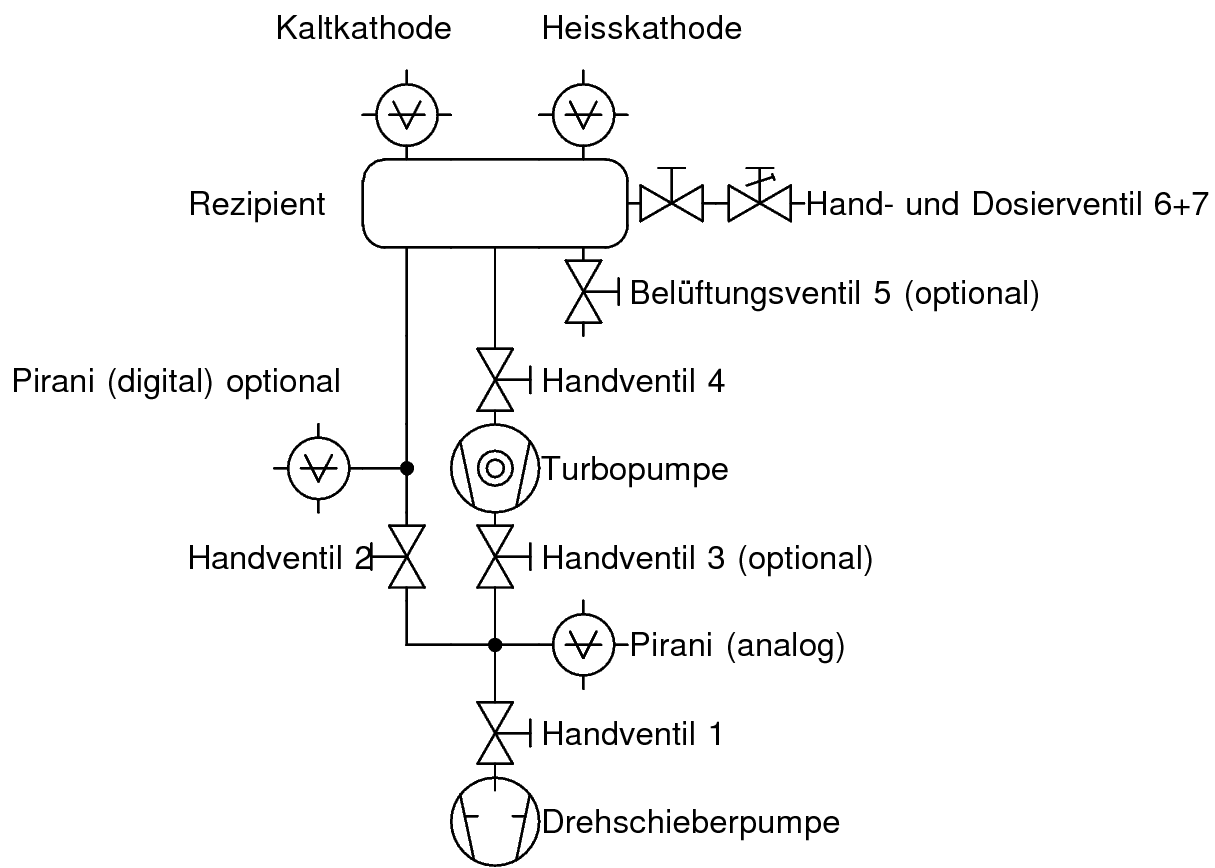
\includegraphics[width=0.8\textwidth]{picture/pumpaufbau.png}
\caption{Schema des Aufbaus des Pumpstandes \cite{Pfeiffer}}
  \label{fig:pump}
\end{figure}
Beim Aufbau des Vakuumstandes wurde darauf geachtet, das Volumen des Systems möglichst gering zu halten, um das System übersichtlich zu halten. Alle Dichtungen sind handfest zugezogen und der Rezipient erwärmt worden, um das Ausgasen zu verringern.
\subsection{Messbereiche}
Aufgrund eines Defekts des Kaltkathodenmessgeräts standen nur das Pirani- sowie, dass Heißkathoden-Messgerät zur Verfügung. Zur Bestimmung der Messgrößen der Drehschieberpumpe wurde deshalb, ausschließlich das Piranimessgerät benutzt, weil aufgrund des Druckbereichs die Glühkathode des Heißkathodenmessgeräts in diesem Bereich kaputt gehen würde. \newline
Zur Bestimmung der Messgrößen der Turbopumpe wurde das Pirani-Messgerät hinter die Drehschieberpumpe geschaltet um zu prüfen ob das entsprechende Vorvakuum zur Inbetriebnahme der Turbopumpe erreicht wurde. Hinter die Turbopumpe wurde anschließend das Glühkathodenmessgerät geschaltet um die Messgrößen des Rezipientens bei der Inbetriebnahme der Turbopumpe zu bestimmen.
\subsection{Messungen an der Drehschiebepumpe}
Zur Bestimmung der Messgrößen der Drehschieberpumpe wird der Versuch wie in Abbildung \ref{fig:Dreh} abgebildet aufgebaut.
\begin{figure}[htpb]
  \centering
  \includegraphics[width=\textwidth]{picture/Aufbau1.png}
  \caption{Pumpstand zur Bestimmung der Kennziffern der Drehschieberpumpe}
  \label{fig:Dreh}
\end{figure}
Der Rezipient (1) wird mittels einer Verbindung (2) anhand eines T-Stückes (5) an ein Ablass-Ventil (3) gekoppelt welches mittels eines Ventils (4) vom Versuch abgeklemmt werden kann. Anschließend folgen zwei T-Stücke (6 \& 8) welche keine gesonderte Funktion haben außer die Kammer um eine Ecke zu lenken. Anschließend folgt ein T-Stück an welchem das Pirani-Messgerät (7) geschaltet ist um den Druck im Rezipienten zu messen. Abschließend folgt ein Ventil (9) um den Rezipienten von der Drehschieberpumpe zu trennen um eine Leckratenmessung durchführen zu können. \newline
Zunächst soll die $p(t)$-Kurve aufgenommen werde. Als erstes wird dafür der Maximaldruck der Drehschieberpumpe gemessen. Dazu muss das Überdruckventil geschlossen werden und der Druck durch die analoge Anzeige des Pirani-Messgerät abgelesen werden. Anschließend wird für vier verschiedene Drücke jeweils zu 18 verschiedenen Drücken die Zeit genommen welche die Pumpe benötigt um diese zu erreichen. Die Messreihe wird jeweils 3-mal durchgeführt. \newline
Anschließend wird die Leckrate bestimmt indem das Überdruckventil so justiert wird, dass sich zwischen Saugvermögen und Luftsstrom ein Gleichgewichtsdruck von (0.1, 0.4, 0.8 und 1.0) \cdot $10^{-2}$ mbar eingestellt. Anschließend wird die Pumpe abgeklemmt und der Druck gegen die Zeit aufgenommen. Dies wird für jeden Gleichgewichtsdruck 5 mal wiederholt.  \newline
\subsection{Turbomolekularpumpe}
Um für die Turbopumpe ein hinreichend großes Vorvakuum zu produzieren muss der Aufbau modifiziert werde. Dafür wird der Zugang zur Drehschieberpumpe vom T-Stück an die Turbopumpe ummontiert und das T-Ventil mit einem Flansch geschlossen. In Abbildung \ref{fig:Turbo} ist der Aufbau zu sehen.
\begin{figure}[htpb]
  \centering
  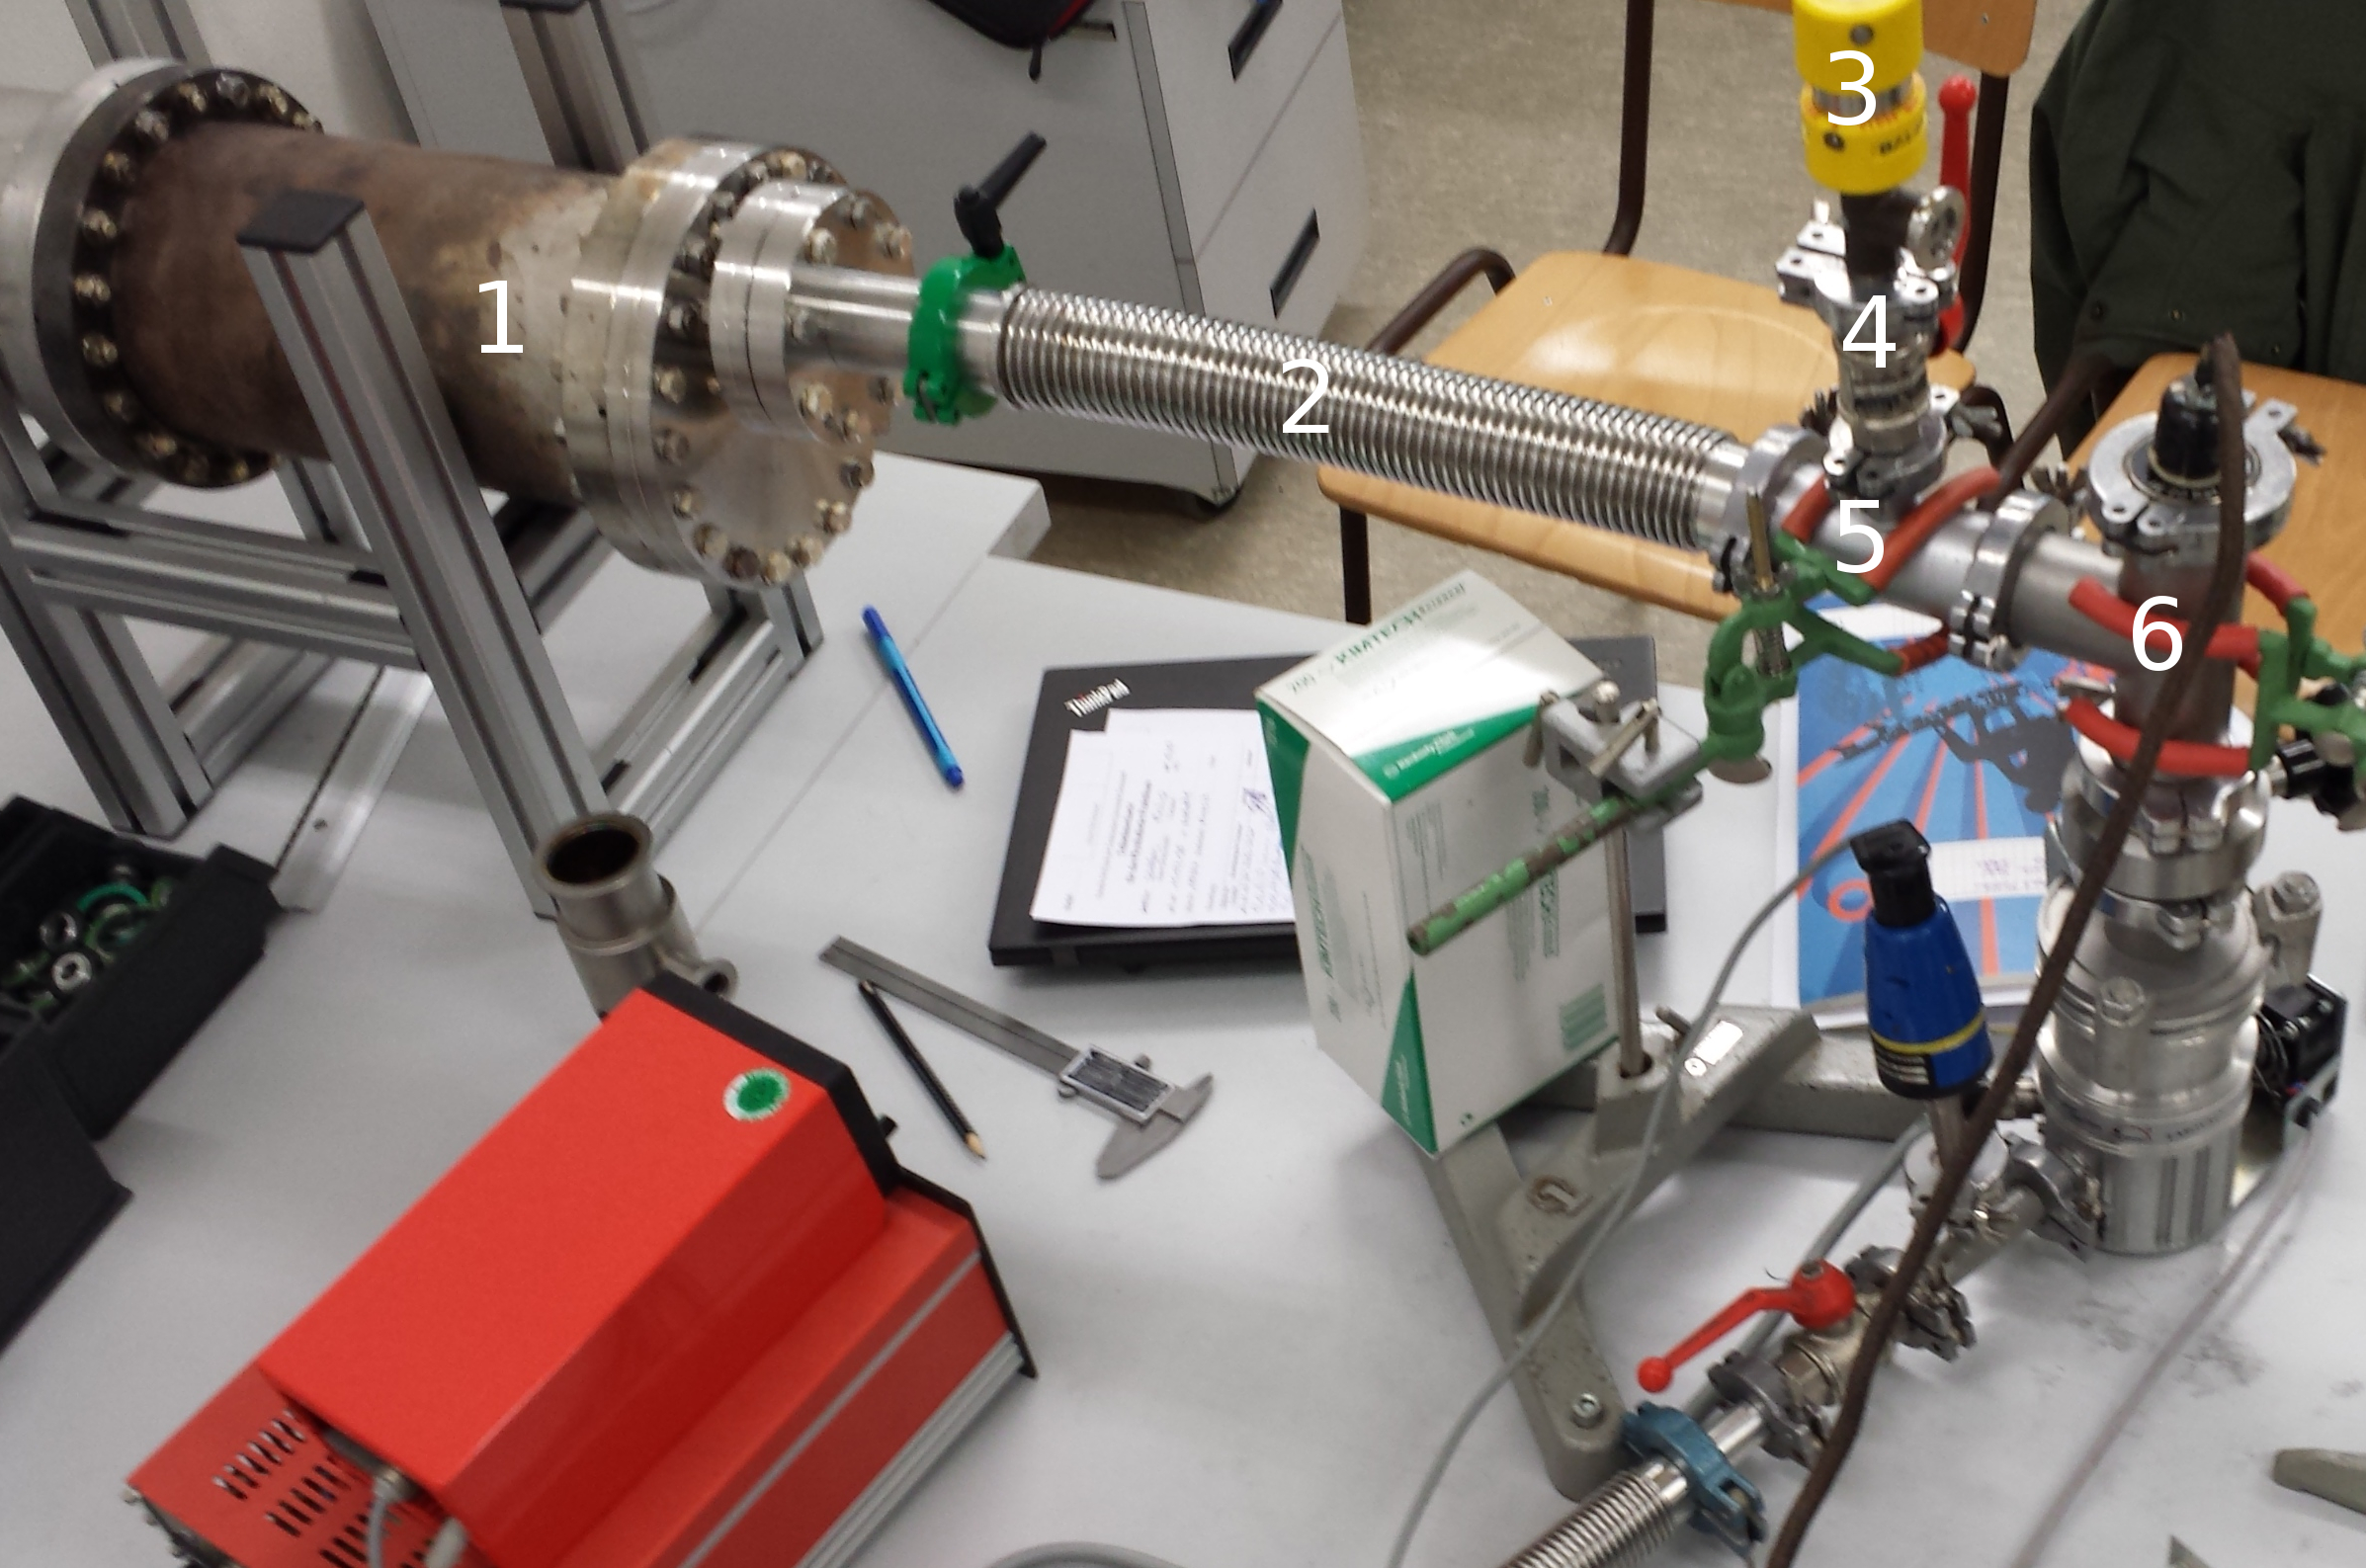
\includegraphics[width=\textwidth]{picture/Aufgabe2.jpg}
  \caption{Aufbau der Turbomolekularpumpe}
  \label{fig:Turbo}
\end{figure}
Anschließend wird die selbe Messreihe wie bei der Drehschiebepumpe aufgenommen, jedoch mit modifizierten Drücken. Es sollen 4 Leckratenmessreihen mit Startdrücken von 5 bis $20 \cdot 10^{-5}$ mbar durchgeführt werden und die $p(t)$-Messung jeweils von einem Druck von $5 \cdot 10^{-3}$ mbar jeweils 3 Messungen. Dabei trat das Problem auf, dass die Glühkathode mit dem Ionenfänger verbunden war und somit die Sicherung des Messgerät vor dem beheben des Problems immer wieder raus sprang. Desweiteren wurden aufgrund der geringen Zeitskalen der Druckverlauf gefilmt und am Computer mittels Movie-Maker ausgewertet, da den Versuchprobanden eine genaue Zeitnahme per Hand nicht möglich schien.
\subsection{Maßentnahme der Objekte}
Zuletzt werden die Maße der Verwendeteten Objekte genommen um das Volumen des evakuierten Raums zu schätzen. Darauf wird der Fehler geschätzt, weil die Innendurchmesser nicht immer mit den Messinstrumenten erreichbar sind.
\subsection{Nachbereitung}
Um das Ausgasen für die folgenden Gruppen zu minimieren wird der Rezipient und alle Pumpen nach beendigung des Versuches mittels eines Flansch geschlossen.
